\documentclass[journal,12pt,twocolumn]{IEEEtran}

\usepackage{setspace}
\usepackage{gensymb}

\singlespacing


\usepackage[cmex10]{amsmath}

\usepackage{amsthm}

\usepackage{mathrsfs}
\usepackage{txfonts}
\usepackage{stfloats}
\usepackage{bm}
\usepackage{cite}
\usepackage{cases}
\usepackage{subfig}

\usepackage{longtable}
\usepackage{multirow}

\usepackage{enumitem}
\usepackage{mathtools}
\usepackage{steinmetz}
\usepackage{tikz}
\usepackage{circuitikz}
\usepackage{verbatim}
\usepackage{tfrupee}
\usepackage[breaklinks=true]{hyperref}
\usepackage{graphicx}
\usepackage{tkz-euclide}
\usepackage{float}

\usetikzlibrary{calc,math}
\usepackage{listings}
    \usepackage{color}                                            %%
    \usepackage{array}                                            %%
    \usepackage{longtable}                                        %%
    \usepackage{calc}                                             %%
    \usepackage{multirow}                                         %%
    \usepackage{hhline}                                           %%
    \usepackage{ifthen}                                           %%
    \usepackage{lscape}     
\usepackage{multicol}
\usepackage{chngcntr}

\DeclareMathOperator*{\Res}{Res}

\renewcommand\thesection{\arabic{section}}
\renewcommand\thesubsection{\thesection.\arabic{subsection}}
\renewcommand\thesubsubsection{\thesubsection.\arabic{subsubsection}}

\renewcommand\thesectiondis{\arabic{section}}
\renewcommand\thesubsectiondis{\thesectiondis.\arabic{subsection}}
\renewcommand\thesubsubsectiondis{\thesubsectiondis.\arabic{subsubsection}}


\hyphenation{op-tical net-works semi-conduc-tor}
\def\inputGnumericTable{}                                 %%

\lstset{
%language=C,
frame=single, 
breaklines=true,
columns=fullflexible
}
\begin{document}


\newtheorem{theorem}{Theorem}[section]
\newtheorem{problem}{Problem}
\newtheorem{proposition}{Proposition}[section]
\newtheorem{lemma}{Lemma}[section]
\newtheorem{corollary}[theorem]{Corollary}
\newtheorem{example}{Example}[section]
\newtheorem{definition}[problem]{Definition}

\newcommand{\BEQA}{\begin{eqnarray}}
\newcommand{\EEQA}{\end{eqnarray}}
\newcommand{\define}{\stackrel{\triangle}{=}}
\bibliographystyle{IEEEtran}
\providecommand{\mbf}{\mathbf}
\providecommand{\pr}[1]{\ensuremath{\Pr\left(#1\right)}}
\providecommand{\qfunc}[1]{\ensuremath{Q\left(#1\right)}}
\providecommand{\sbrak}[1]{\ensuremath{{}\left[#1\right]}}
\providecommand{\lsbrak}[1]{\ensuremath{{}\left[#1\right.}}
\providecommand{\rsbrak}[1]{\ensuremath{{}\left.#1\right]}}
\providecommand{\brak}[1]{\ensuremath{\left(#1\right)}}
\providecommand{\lbrak}[1]{\ensuremath{\left(#1\right.}}
\providecommand{\rbrak}[1]{\ensuremath{\left.#1\right)}}
\providecommand{\cbrak}[1]{\ensuremath{\left\{#1\right\}}}
\providecommand{\lcbrak}[1]{\ensuremath{\left\{#1\right.}}
\providecommand{\rcbrak}[1]{\ensuremath{\left.#1\right\}}}
\theoremstyle{remark}
\newtheorem{rem}{Remark}
\newcommand{\sgn}{\mathop{\mathrm{sgn}}}
\providecommand{\abs}[1]{\lvert#1\vert}
\providecommand{\res}[1]{\Res\displaylimits_{#1}} 
\providecommand{\norm}[1]{\lVert#1\rVert}
%\providecommand{\norm}[1]{\lVert#1\rVert}
\providecommand{\mtx}[1]{\mathbf{#1}}
\providecommand{\mean}[1]{E[ #1 ]}
\providecommand{\fourier}{\overset{\mathcal{F}}{ \rightleftharpoons}}
%\providecommand{\hilbert}{\overset{\mathcal{H}}{ \rightleftharpoons}}
\providecommand{\system}{\overset{\mathcal{H}}{ \longleftrightarrow}}
	%\newcommand{\solution}[2]{\textbf{Solution:}{#1}}
\newcommand{\solution}{\noindent \textbf{Solution: }}
\newcommand{\cosec}{\,\text{cosec}\,}
\providecommand{\dec}[2]{\ensuremath{\overset{#1}{\underset{#2}{\gtrless}}}}
\newcommand{\myvec}[1]{\ensuremath{\begin{pmatrix}#1\end{pmatrix}}}
\newcommand{\mydet}[1]{\ensuremath{\begin{vmatrix}#1\end{vmatrix}}}
\numberwithin{equation}{subsection}
\makeatletter
\@addtoreset{figure}{problem}
\makeatother
\let\StandardTheFigure\thefigure
\let\vec\mathbf
\renewcommand{\thefigure}{\theproblem}
\def\putbox#1#2#3{\makebox[0in][l]{\makebox[#1][l]{}\raisebox{\baselineskip}[0in][0in]{\raisebox{#2}[0in][0in]{#3}}}}
     \def\rightbox#1{\makebox[0in][r]{#1}}
     \def\centbox#1{\makebox[0in]{#1}}
     \def\topbox#1{\raisebox{-\baselineskip}[0in][0in]{#1}}
     \def\midbox#1{\raisebox{-0.5\baselineskip}[0in][0in]{#1}}
\vspace{3cm}
\title{Assignment 3}
\author{Unnati Gupta}
\maketitle
\newpage
\bigskip
\renewcommand{\thefigure}{\theenumi}
\renewcommand{\thetable}{\theenumi}
Download all python codes from 
\begin{lstlisting}
https://github.com/unnatigupta2320/Assignment_3/tree/master/CODES
\end{lstlisting}
%
and latex-tikz codes from 
%
\begin{lstlisting}
https://github.com/unnatigupta2320/Assignment_3
\end{lstlisting}
%
\section{Question No. 2.59}
Draw a line segment $\vec{AB}$ of length 8 units. Taking $\vec{A}$ as centre draw a circle of radius $4$ units and taking $\vec{B}$ as centre draw a circle of radius $3$ units. Construct tangents to each circle from the centre of other circle.

%
\section{Solution}
Given that, line segment $AB$=8 units.So,Let:
\begin{align}
\vec{A}=\myvec{a\\0}=\myvec{0\\0} 
\\
\vec{B}=\myvec{b\\0}=\myvec{8\\0}    
\end{align} 
\\
Further the given data is tabularised in table \ref{tab:table1}:
\numberwithin{table}{section}
\begin{table}[!ht]
\begin{center}
\begin{tabular}{ | m{2cm} | m{1.5cm}| m{2cm} | m{1.5cm} |} 
\hline
 & Symbols & Circle1 & Circle2 \\
\hline
Centre & $\vec{O}$ & \myvec{0\\0} & \myvec{8\\0} \\ 
\hline
Radius & $r_{1}$,$r_{2}$ & 4 & 3 \\ 
\hline
Polar coordinates & $\vec{C}_{1}$,$\vec{C}_{2}$ & 4\myvec{\cos \theta\\  \sin \theta} & 3\myvec{\cos \theta\\  \sin \theta} \\
\hline
Angle & $\theta$ & 0-2$\pi$ & 0-2$\pi$ \\
\hline
\end{tabular}
\end{center}
\caption{Input values}
\label{tab:table1}
\end{table}
\begin{enumerate}
    \item For tangents at \textbf{Circle1} from $\vec{B}$:-
\begin{itemize}
\item Let $BP$ and $BQ$  be tangents to \textbf{Circle1} with radius 4 units.
\item We know a tangent is always perpendicular to the radius .
\begin{align}
\therefore AP \perp BP ,  AQ \perp BQ.
\end{align}
\item Now,
\begin{align}
 \implies (\vec{A}-\vec{P})^T (\vec{B}-\vec{P}) &= 0 \quad \brak{\because AP \perp BP }
 \\
 \implies\vec{P}^T(\vec{B}-\vec{P})&= 0 \quad \brak{\because \vec{A}=0}
 \\
  \implies\vec{P}^T \vec{B} - \vec{P}^T \vec{P} &= 0  
  \\
  \implies\norm{\vec{P}}^2 &= \vec{P}^T \vec{B}
  \\
 \implies \norm{\vec{P}}^2 &= \vec{B}^T \vec{P} 
  \\
  \implies \vec{B}^T \vec{P} &= 16 \quad \brak{\because \norm{\vec{P}}^2 = 16}
  \\
  \implies \myvec{8&0} \vec{P} &= 16 \quad \brak{\because \vec{B} = \myvec{8\\0} }
  \\
   \implies\myvec{1&0} \vec{P} &= 2
   \\
   \implies\vec{P} &= \myvec{2\\0} + \lambda \myvec{0\\1} 
    \end{align}
    \begin{align}
    \implies \vec{P}&=\vec{p}+\lambda\vec{m} \label{eqa}
   \\
   \text{where, }\vec{p}&=\myvec{2\\ 0}
   \\
   \text{and }\vec{m}&=\myvec{0\\1}
\end{align}
\item We know,
\begin{align}
\norm{\vec{p}+\lambda\vec{m}}^2&=16
\\
(\vec{p}+\lambda \vec{m})^T(\vec{p}+\lambda \vec{m})&=16
\\
\lambda^2&=\frac{16-\norm{\vec{p}}^2}{\norm{\vec{m}}^2}
\end{align}
\begin{align}
  \lambda = \pm 3.46  
\end{align}


Substitute $\lambda$  value in \eqref{eqa} we get the coordinates of $\vec{P}$ and  $\vec{Q}$ as :
\begin{align}
\vec{P}=\myvec{2\\3.46},
\vec{Q}=\myvec{2\\-3.46}
\end{align}
\end{itemize}

\item For tangents at \textbf{Circle2} from $\vec{A}$:-
\begin{itemize}
\item In $\triangle$ ABR, using Pythagoras Theorem,we get:
\begin{align}
    \norm{\vec{A}-\vec{B}}^2 &= \norm{\vec{A}-\vec{R}}^2+ \norm{\vec{B}-\vec{R}}^2
    \\
    \norm{\vec{A}-\vec{R}}^2 &=\norm{\vec{A}-\vec{B}}^2 - \norm{\vec{B}-\vec{R}}^2
    \end{align}
    \item As, $\vec{A}=0$, above equation get reduced to:
    \begin{align}
    \norm{\vec{R}}^2 = \norm{\vec{A}-\vec{B}}^2 - \norm{\vec{B}-\vec{R}}^2 
    \\
    \norm{\vec{R}}^2= 8^2 -3^2=55 \label{eqc}
\end{align}
\end{itemize}
\item Let $AR$ and $AS$  be tangents to \textbf{Circle2} with radius 3 units.
\begin{itemize}
\item We know a tangent is always perpendicular to the radius .
\begin{align}
\therefore AR \perp BR ,  AS \perp BS.
\end{align}
\item Now,
\begin{align}
 \implies (\vec{A}-\vec{R})^T (\vec{B}-\vec{R}) &= 0 \quad \brak{\because AR \perp BR }
 \\
 \implies\vec{R}^T(\vec{B}-\vec{R})&= 0 \quad \brak{\because \vec{A}=0}
 \\
  \implies\vec{R}^T \vec{B} - \vec{R}^T \vec{R} &= 0  
  \\
  \implies\norm{\vec{R}}^2 &= \vec{R}^T \vec{B}
  \\
 \implies \norm{\vec{R}}^2 &= \vec{B}^T \vec{R} 
  \end{align}
  \item Now, we have $\norm{\vec{R}}^2 =55$, putting the value in above equation we get:
  \begin{align}
  \implies \vec{B}^T \vec{R} &= 55 
  \\
  \implies \myvec{8&0} \vec{R} &= 55 \quad \brak{\because \vec{B} = \myvec{8\\0} }
  \\
   \implies\myvec{1&0} \vec{R} &= \frac{55}{8}
   \\
   \implies\vec{R} &= \myvec{\frac{55}{8}\\0} + \mu \myvec{0\\1} 
    \\
    \implies \vec{R}&=\vec{r}+\mu\vec{m} \label{eqb}
   \\
   \text{where, }\vec{r}&=\myvec{\frac{55}{8}\\0}
   \\
   \text{and }\vec{m}&=\myvec{0\\1}
\end{align}
\item We know,
\begin{align}
\norm{\vec{r}+\mu\vec{m}}^2&=55
\\
(\vec{r}+\mu \vec{m})^T(\vec{r}+\mu \vec{m})&=55
\\
\mu^2&=\frac{55-\norm{\vec{r}}^2}{\norm{\vec{m}}^2}
\\
\mu &= \pm 2.78
\end{align}
Substitute $\mu$  value in \eqref{eqb} we get the coordinates of $\vec{R}$ and  $\vec{S}$ as :
\begin{align}
\vec{R}=\myvec{6.875\\2.78},
\vec{S}=\myvec{6.875\\-2.78}
\end{align}
\end{itemize}
\end{enumerate}

\numberwithin{figure}{section}
\begin{figure}[H]
\centering
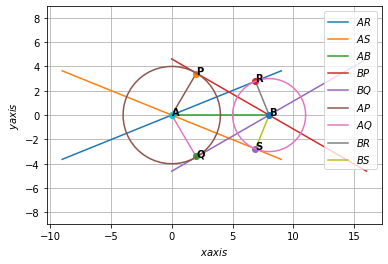
\includegraphics[width=\columnwidth]{Tangents on Circles with Centre A and B.png}
\caption{Tangents from centres of Circle}
\label{fig:circle}	
\end{figure}
\end{document}